\documentclass[12pt]{article}
\usepackage{graphicx}
\usepackage{commath}
\usepackage{gensymb}
\usepackage{float}

\begin{document}
\begin{center}
\textbf\large{CHAPTER-7 \\ COORDINATE GEOMETRY}
\end{center}

\section{EXERCISE - 7.1}
\begin{enumerate}
\item Find the distances between the following pairs of points:
\begin{enumerate}
\item $(2,3),(4,1)$
\item $(-5,7),(-1,3)$
\item $(a,b),(-a,-b)$
\end{enumerate}
\item Find the distance between the points $(0,0) and (36,15)$,Can you now find the distances between the two towns A and B discussed in Section 7.2 .
\item Determine if the points$(1,5),(2,3) and (-2,-11)$ are collinear.
\item Check whether$(5,-2),(6,4)and (7,-2)$ are the vertices of an isosceles triangle.
\item  In a classroom, 4 friends are seated at the points A,B,C and D as shown in Fig. 7.8, Champa and Chameli walk in to the class and after observing for a few minutes Champa asks Chameli,"Dont't you think ABCD is a square?" Chameli disagrees,Using distance formula, find which of them is correct.

\begin{figure}[!h]
\centering
  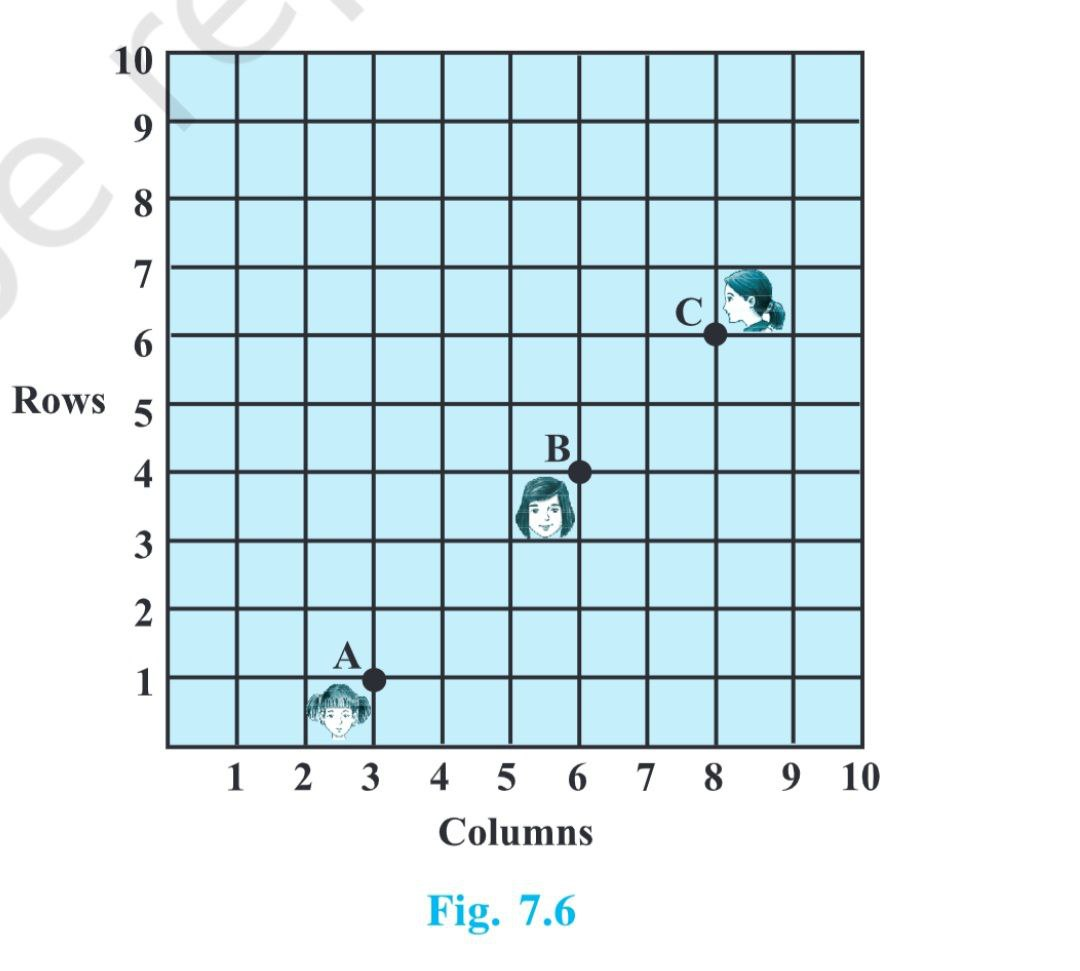
\includegraphics[width=\columnwidth]{canvas.jpg}
 \caption{}
\label{fig:10/7/4/8Fig3}
\end{figure}

\item Name the type of quadrilateral formed,if any,by the following points,and give reasons for your answer:
\begin{enumerate}
\item $(-1,-2),(1,0),(-1,2),(-3,0)$
\item $(-3,5),(-3,1),(0,3),(-1,-4)$
\item $(4,5),(7,6),(4,3),(1,2)$
\end{enumerate}
\item Find the point on the x-axis which is equidistant from$(2,-5)$and$(-2,9)$.
\item Find the values of y for which the distance between the points                  $\vec{P}P(2,-3)and \vec{Q}Q(10,y)$is10 units.
\item  If $Q(0, 1)$ is equidistant from $P(5, –3) and R(x, 6)$, find the values of x. Also find the
distances QR and PR.
\item  Find a relation between x and y such that the point $(x, y)$ is equidistant from the point
$(3, 6) and (– 3, 4)$.

\end{enumerate}

\end{document}
